\maketitle
\vspace{-2\baselineskip}

\setcounter{tocdepth}{2}
\tableofcontents
\thispagestyle{empty}
\vspace{0.6\baselineskip}

\section{Proxmox VEとは}

{\small
\begin{itemize}[topsep=0pt,itemsep=0pt,parsep=0pt,partopsep=0pt]
\item ProxmoxVEはDebianベースの仮想化基盤\cite{proxmox-ve}
\item WebGUIでの直感的な操作が特徴的で、数回ボタンをクリックするだけですぐVM,LXCコンテナを建てることができる
\item 思う存分サービスを破壊できる
\item 無料で使える（嬉）
\end{itemize}
}

\termdefs{※ VM: 仮想マシン。LXC: 軽量なLinuxコンテナ。VLAN: 1本の物理ネットワークを用途別に論理分割する仕組み。}

\section{この記事を書いた理由}

自宅鯖/Proxmoxを布教したい（盆栽的な楽しさがあります）。最近、自宅鯖をいじっていたときにいろいろあってノードごと破壊したので、組み直すついでにインストールから運用までをまとめました。

\section{Proxmox VEのインストール}

\subsection{インストール前に用意するもの}

\begin{itemize}
\item \textsf{\textbf{物理マシン}}：x86-64マシンなら基本何でも良い。ただし、VMを動かすには仮想化支援機能（Intel VT-x / AMD-V）が有効になっている必要があります。最近は企業から払い下げられたシンクライアント（富士通のFUTROやDELLのWyseなど）を買ってきてクラスタを組む人をよく見ます（kawaii）。
\qritem{起動用USBメモリ}{https://www.proxmox.com/en/downloads/proxmox-virtual-environment/iso}{リンクからISOを落とし（2026年時点ではV9.2が最新）、Balena EtcherなどでUSBメモリに書き込む。}
\item \textsf{\textbf{NIC}}：基本はオンボードで十分。10G回線と10Gスイッチがあるなら、X520-DA2などの10G NIC（図\ref{fig:x520-da2}）を足すと高速になって良い。
\item \textsf{\textbf{管理用PC}}：ProxmoxのWeb UIに入るためのPC。ブラウザが動けば何でも良い。
\item \textsf{\textbf{モニター}}：セットアップ時に使用。
\end{itemize}

\installfigure[0.38\linewidth]{media/homelab/x520-da2.jpg}{X520-DA2。Aliexpressで5千円ぐらいで手に入ります。}{fig:x520-da2}


\subsection{インストールする}

Proxmox VEのISOをUSBメモリへ書き込み、USBから起動します。

起動時に各機種のブートメニューを開き、Proxmox VEを書き込んだUSBメモリを選びます。

\installfigrow[0.94\linewidth]{media/proxmox-installation/03-proxmox-installer-menu.png}{Proxmox VE 9.2のインストールメニュー。この画面まで来たら \texttt{Install Proxmox VE (Graphical)} を選びます。}{fig:proxmox-installer-menu}{media/proxmox-installation/04-target-disk.png}{インストール先ディスクの選択。対象ディスクは初期化されます。}{fig:target-disk}

画面に従って地域、タイムゾーン、キーボード配列、rootパスワード、通知用メールアドレスを設定します。

\installfigrow{media/proxmox-installation/06-management-network.png}{管理ネットワーク設定。ProxmoxのWeb UIにアクセスするためのIPアドレスを、環境に合わせて設定してください。このあとのSummary画面で設定を確認してInstallを押します。}{fig:management-network}{media/proxmox-installation/07-console-url-cropped.png}{インストール完了後のコンソール。\texttt{https://先ほど設定したIPv4アドレス:8006/} が表示されれば、管理PCからProxmox VEのWeb UIへ入る準備ができています。}{fig:console-url}

インストール後は、管理PCのブラウザから表示されたURLにアクセスします。rootユーザーでログインして、次のようなWeb UIが表示されればインストールは成功です。

\installfigure[0.50\linewidth]{media/proxmox-installation/09-proxmox-webui-after-login.png}{ブラウザからProxmox VEのWeb UIへ入った状態。}{fig:proxmox-webui}

\subsection{初期セットアップをする}

まず、サブスクリプションなしでもアップデートが止まらないよう、Proxmox VE Helper-Scriptsの \texttt{PVE Post Install} でリポジトリを整えます\cite{proxmox-helper-scripts}。Enterpriseリポジトリの無効化、No-Subscriptionリポジトリの有効化、subscription nagの抑制、Proxmox VEの更新までを対話式でまとめて済ませられます。

\begin{commands}
# ProxmoxホストのShellで初期セットアップを対話実行する。
bash -c "$(curl -fsSL https://raw.githubusercontent.com/community-scripts/ProxmoxVE/main/tools/pve/post-pve-install.sh)"
\end{commands}

\siteqrcode{PVE Post Install}{https://community-scripts.org/scripts/post-pve-install}

質問には次の方針で答えます。
\begin{enumerate}
\item \texttt{Start the Proxmox VE Post Install Script (y/n)?} で \texttt{y} を選ぶ。
\item \texttt{pve-enterprise} と \texttt{ceph enterprise} は \texttt{disable}、\texttt{pve-no-subscription} は \texttt{yes}、\texttt{pve-test} は不要なら \texttt{no} を選ぶ。
\item subscription nagは \texttt{yes} で無効化し、\texttt{Disable high availability?} は \texttt{no} を選ぶ。
\item Proxmox VEの更新と再起動は、どちらも \texttt{yes} を選ぶ。
\end{enumerate}

\subsection{おすすめの使い方}

Proxmox VE Helper-Scriptsは、初期セットアップだけでなく、VM/LXCを作るときにも便利です\cite{proxmox-helper-scripts}。おすすめを6つに絞ります。
\siteqrcode{Proxmox VE Helper-Scripts}{https://community-scripts.github.io/ProxmoxVE/}

\begin{description}
\item[Docker VM] DockerをVMで動かす。LXC派閥もいて、どちらが良いのやら…
\item[Home Assistant OS] 家電、センサー、スマートプラグなどをまとめる。
\item[AdGuard Home] 家庭内DNSと広告ブロックに使う。設定はkatori\_m氏の記事を参照\cite{katori-adguard-home}。
\item[Tailscale LXC] 外出先からのリモートアクセスに使う。
\item[Cloudflared] ポート開放せずサービスを公開する。我が家ではMinecraftサーバーに使用。
\item[Zabbix] サーバーやネットワークを監視し、見ながらﾆﾁｬﾆﾁｬする。
\end{description}

\termdefs{※ Docker: アプリをコンテナとして動かす仕組み。\\
※ DNS: 名前からIPアドレスを引く仕組み。\\
※ Cloudflare Tunnel: 自宅側からCloudflareへ接続してサービスを公開する仕組み。}

\section{自宅鯖弄り録}

Proxmoxのユースケースとして、我が家の環境を組み直したときの作業をまとめました。

役に立つかは謎です。


% 構成図と写真2点はセクション導入の直後に置く。写真は枚数を保ったまま横並びにする。
\begin{figure}[H]
  \centering
  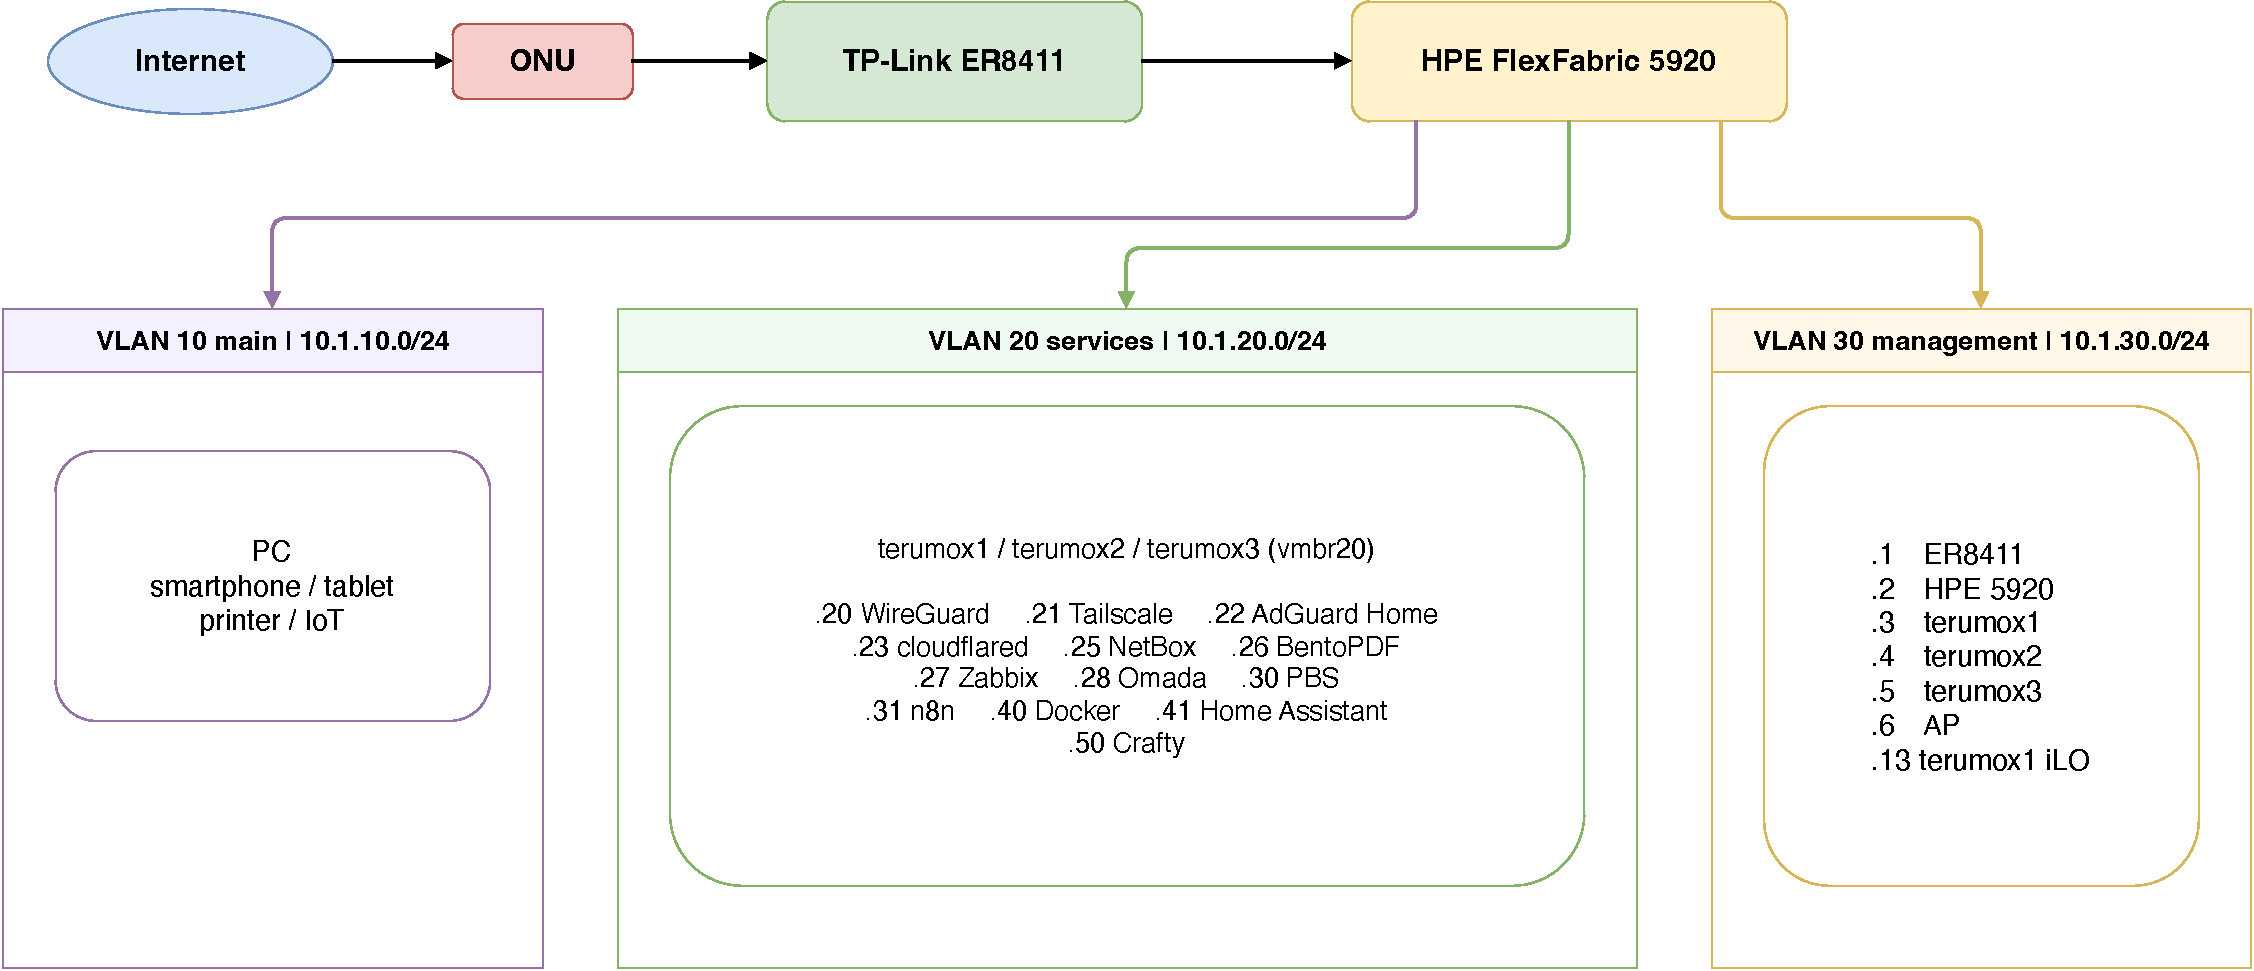
\includegraphics[width=\linewidth]{media/diagrams/home-network-final.pdf}
  \caption{我が家の構成}
  \label{fig:home-network-current}
\end{figure}

\begin{figure}[H]
  \centering
  \begin{minipage}[t]{0.48\linewidth}
    \centering
    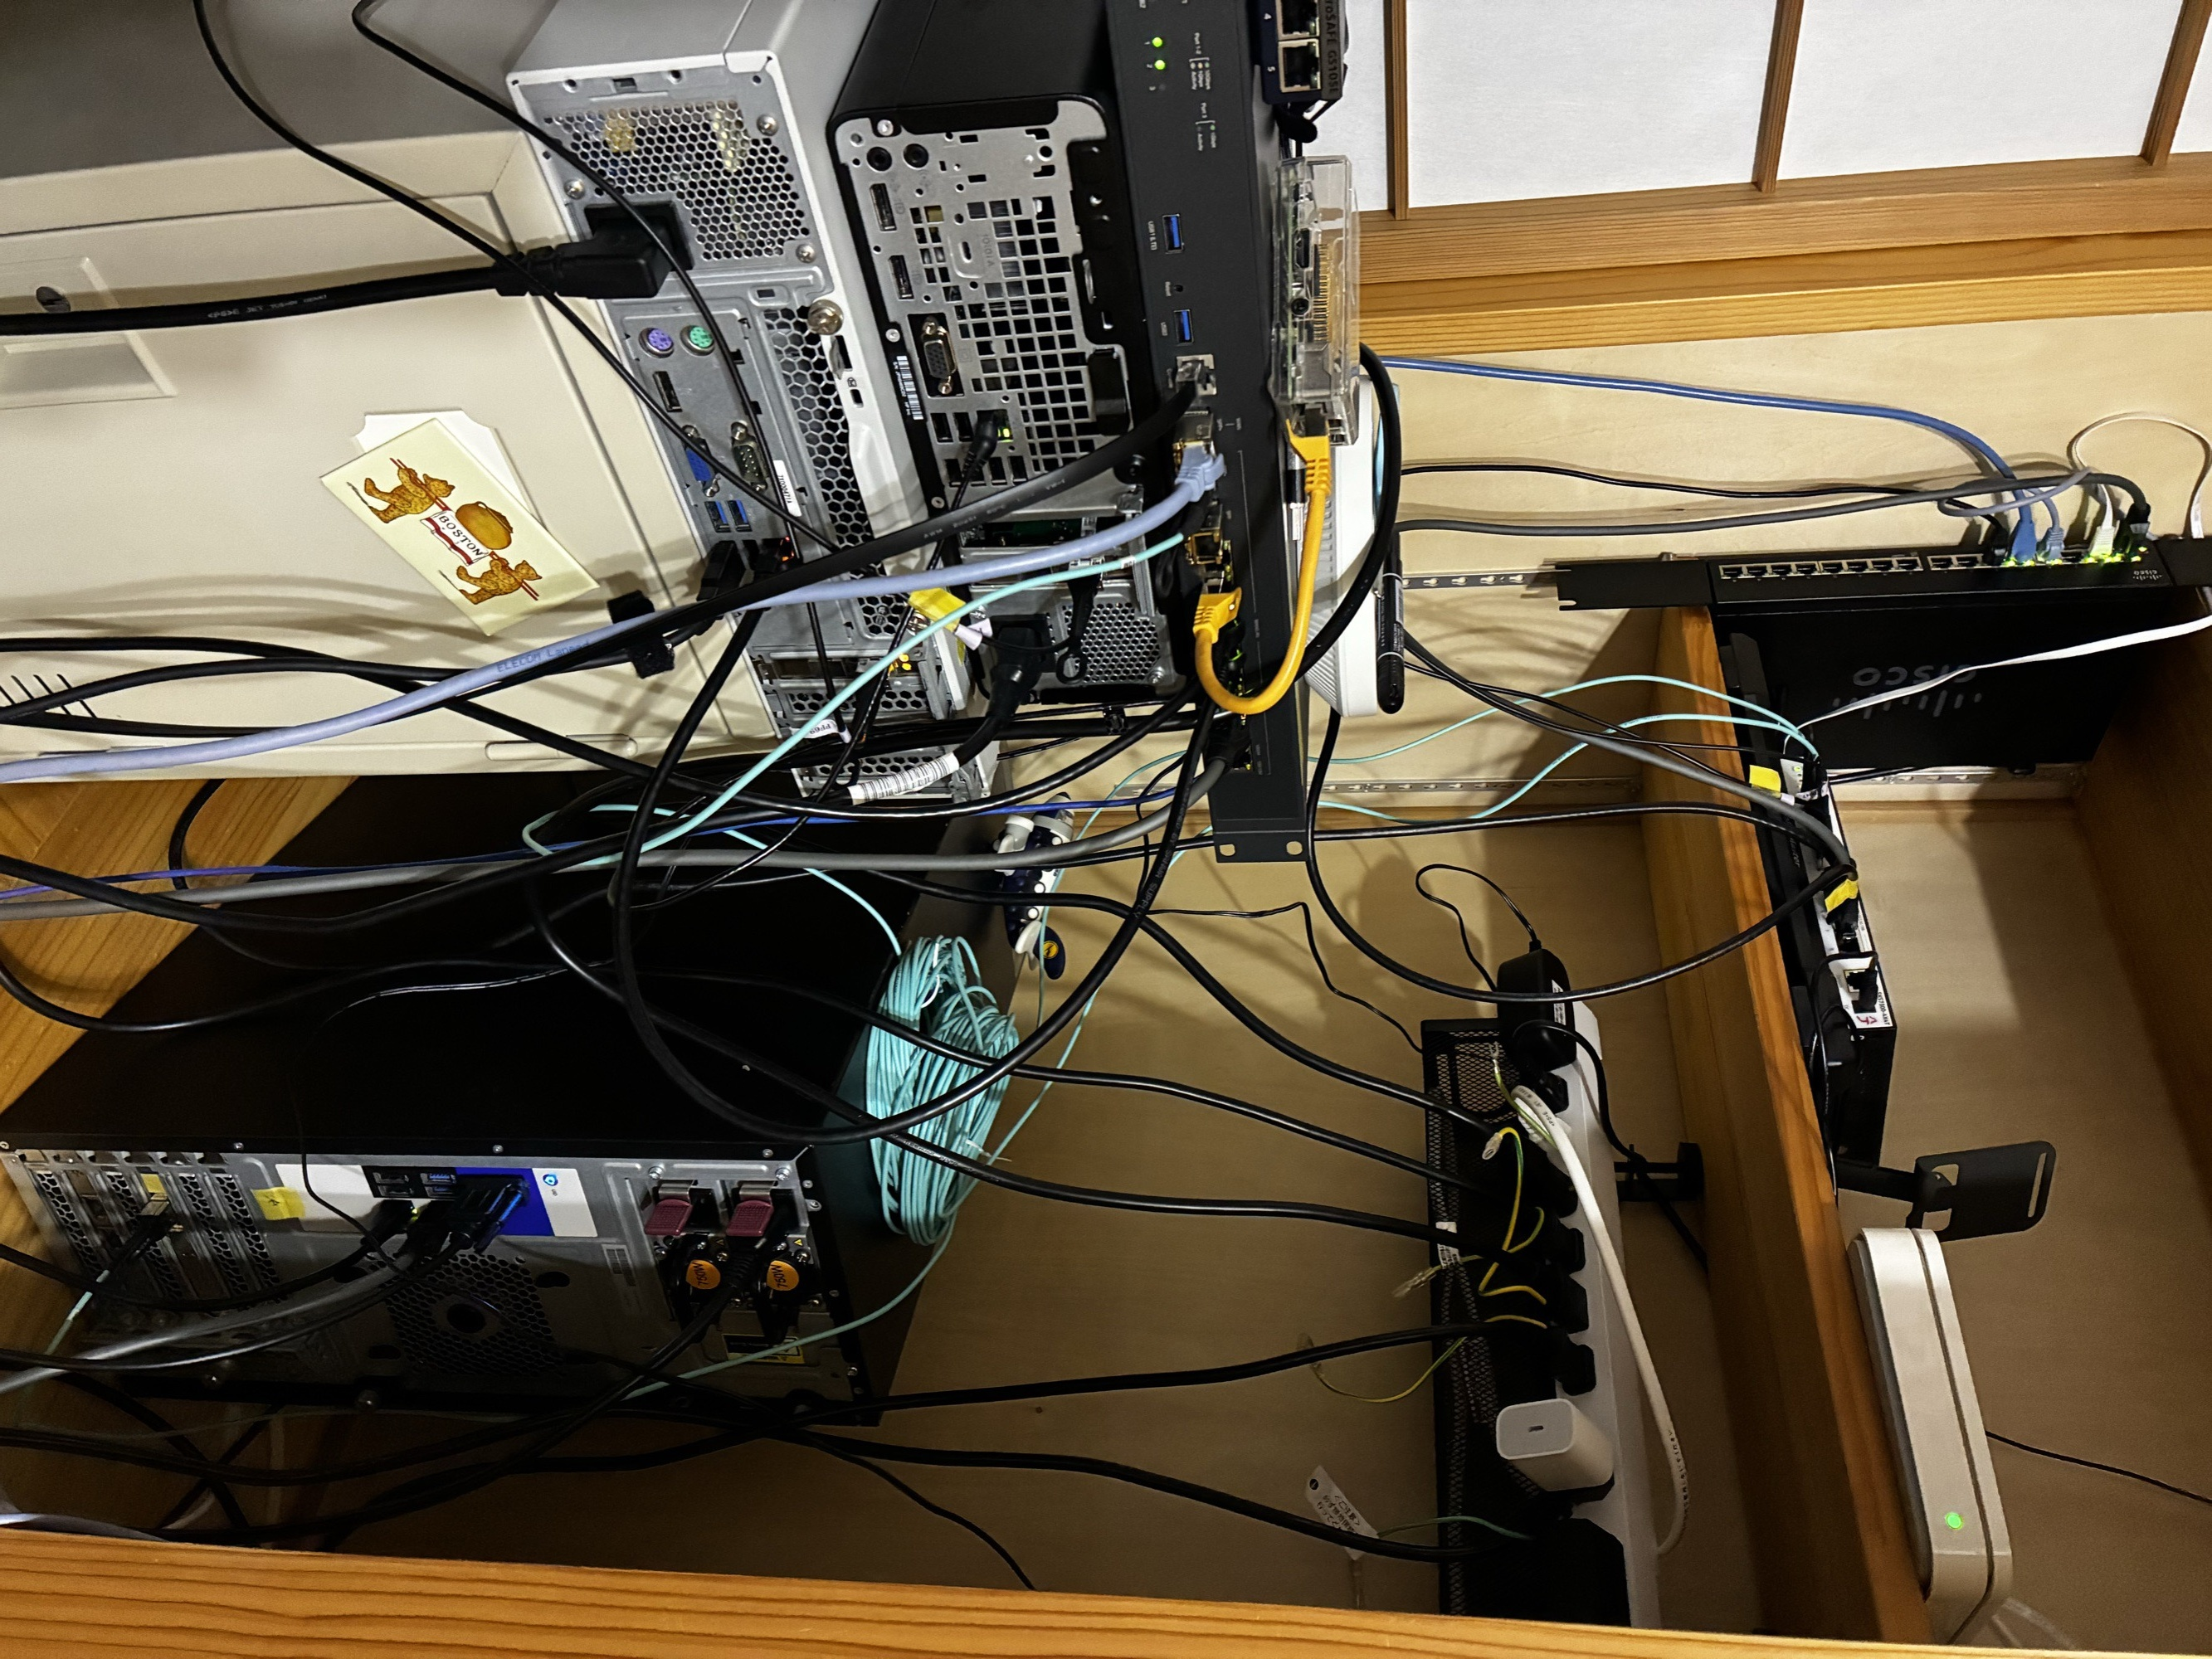
\includegraphics[width=\linewidth,height=0.23\textheight,keepaspectratio]{media/homelab/server-shelf.jpg}
    \caption{我が家のサーバー群。撮影後にコアスイッチの電源が溶けたので入れ替えました。}
    \label{fig:server-shelf}
  \end{minipage}\hfill
  \begin{minipage}[t]{0.48\linewidth}
    \centering
    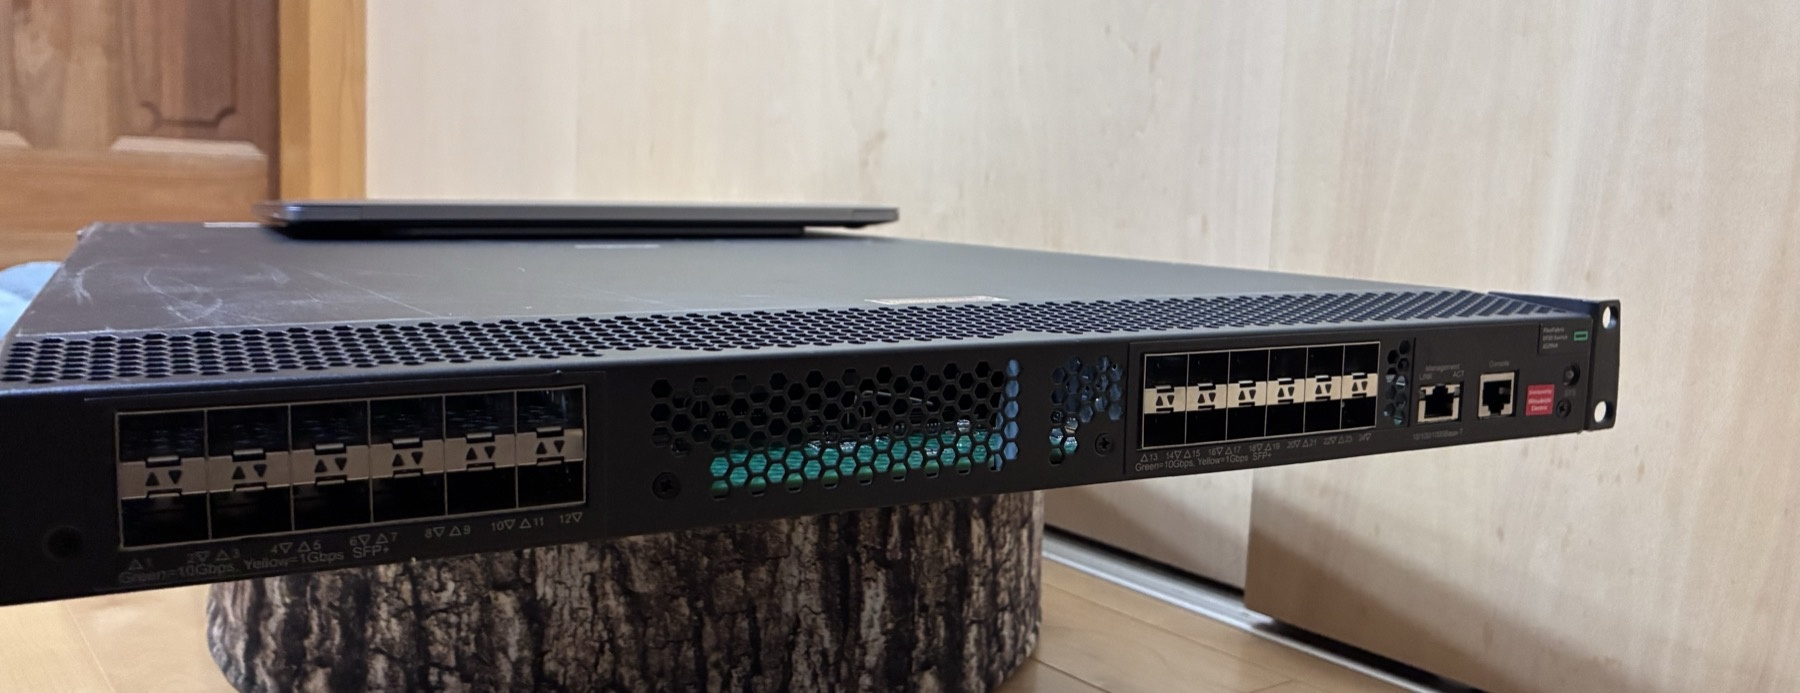
\includegraphics[width=\linewidth,height=0.23\textheight,keepaspectratio]{media/homelab/hpe-core-switch.jpg}
    \caption{新コアスイッチ、HPE FlexFabric 5920（SFP+×24）。うるさすぎる。}
    \label{fig:hpe-core-switch}
  \end{minipage}
\end{figure}

\subsection{用途ごとにVLANで区切る}

役割ごとにVLANで区切って運用しやすいようにします。普段使いはVLAN 10、サービスはVLAN 20、インフラ管理はVLAN 30に分けました。

\begin{center}
\begin{tabular}{@{}ll@{}}
\textsf{\textbf{VLAN 10（main）}} & \texttt{10.1.10.0/24}、gateway \texttt{10.1.10.1} \\
\textsf{\textbf{VLAN 20（services）}} & \texttt{10.1.20.0/24}、gateway \texttt{10.1.20.1} \\
\textsf{\textbf{VLAN 30（management）}} & \texttt{10.1.30.0/24}、gateway \texttt{10.1.30.1} \\
\textsf{\textbf{管理スイッチ}} & \texttt{10.1.30.2} \\
\textsf{\textbf{terumox1 Proxmox}} & \texttt{10.1.30.3} \\
\textsf{\textbf{terumox2 Proxmox}} & \texttt{10.1.30.4} \\
\textsf{\textbf{terumox3 Proxmox}} & \texttt{10.1.30.5} \\
\end{tabular}
\end{center}

内部DNSの\termmark{ドメイン}は、\termmark{Bonjour/mDNS}の \texttt{.local} と衝突しないよう \texttt{home.arpa} にします。\texttt{ha.home.arpa}、\texttt{crafty.home.arpa}、\texttt{mc.home.arpa} のようになります。
\termdefs{※ ドメイン: 名前解決で使う名前のまとまり。\\
※ Bonjour/mDNS: 同一LAN内で機器名を自動発見する仕組み。}

\subsection{クラスタを作る}

quorum（過半数のノードが稼働している状態）を確保するため3台構成にしています。2台だと1台落ちた時点で過半数を割りますが、3台なら1台落ちても残り2台で保てます。

まず名前解決を揃えます。画面に出てくる \texttt{Link 0} は、Corosync（クラスタ管理の仕組み）がノード間通信に使う経路です。ノード名とIPの対応がずれていると参加に失敗するため、先に3台すべての \texttt{/etc/hosts} へ同じ3行を入れて固定しました。

\begin{commands}
# 3台すべての /etc/hosts に入れ、ノード名を管理VLANのIPへ固定する。
10.1.30.3 terumox1.home.arpa terumox1
10.1.30.4 terumox2.home.arpa terumox2
10.1.30.5 terumox3.home.arpa terumox3
\end{commands}

なお、Proxmoxの公式ドキュメントではCorosyncのlink addressにIPアドレスを直接使う方が安全とされています。Web UIで明示的にIPを選べる場合は選んでおきましょう。

名前解決が揃ったら、1台目でクラスタを作成します。\texttt{terumox1} のWeb UIで「データセンター」→「クラスタ」を開き、「クラスタを作成」を押します。\texttt{クラスタ名} に \texttt{terumox-cluster} を入れ、\texttt{Link 0} には管理VLANのIP \texttt{10.1.30.3} を選んで「作成」を押します。

作成できたら、同じ画面の「Join情報」を開き、「情報をコピー」で丸ごとコピーしておきます。

続いて \texttt{terumox2}、\texttt{terumox3} を順番に参加させます。ノードのWeb UIで「クラスタ」→「クラスタに参加」を開き、Join情報を「情報」欄へ貼り付けると \texttt{Peerアドレス} と \texttt{指紋} が自動で埋まります。あとは \texttt{terumox1} の \texttt{root} パスワードを入力し、\texttt{Link 0} にそのノード自身の管理VLAN IP（\texttt{terumox2} なら \texttt{10.1.30.4}）を選んで参加します。

実際の作業では、\texttt{terumox3} の参加が途中で失敗しました。\texttt{pvecm status} で半端な登録を確認し、失敗ノードを削除して参加をやり直すことで復旧しました。削除の手順は既存の実例を参考にしました\cite{wildrick-proxmox-cluster-remove}。

\installfigure[0.66\linewidth]{media/cluster/04-cluster-datacenter-summary.png}{クラスタ作成後のデータセンター画面。\texttt{terumox1}〜\texttt{terumox3}の3ノードが\texttt{terumox-cluster}として1つにまとまっています。}{fig:cluster-summary}

\subsection{管理スイッチを設定する}

スイッチ側では、先に決めたVLANを作成し、接続先に応じて各ポートの役割を設定します。設定画面やコマンドは機種ごとに異なるため、ここでは設定の内容だけ大まかに書きます。収容例を図\ref{fig:managed-switch-vlan-overview}に示します。

% この図は手順に縛られない説明図なので、ページを跨ぐ余白を作らないようフロートにする。
% 直前の[H]図（クラスタ画面）より上に浮いて図番号の順序が逆転しないよう、下部配置に限定する。
\begin{figure}[!b]
  \centering
  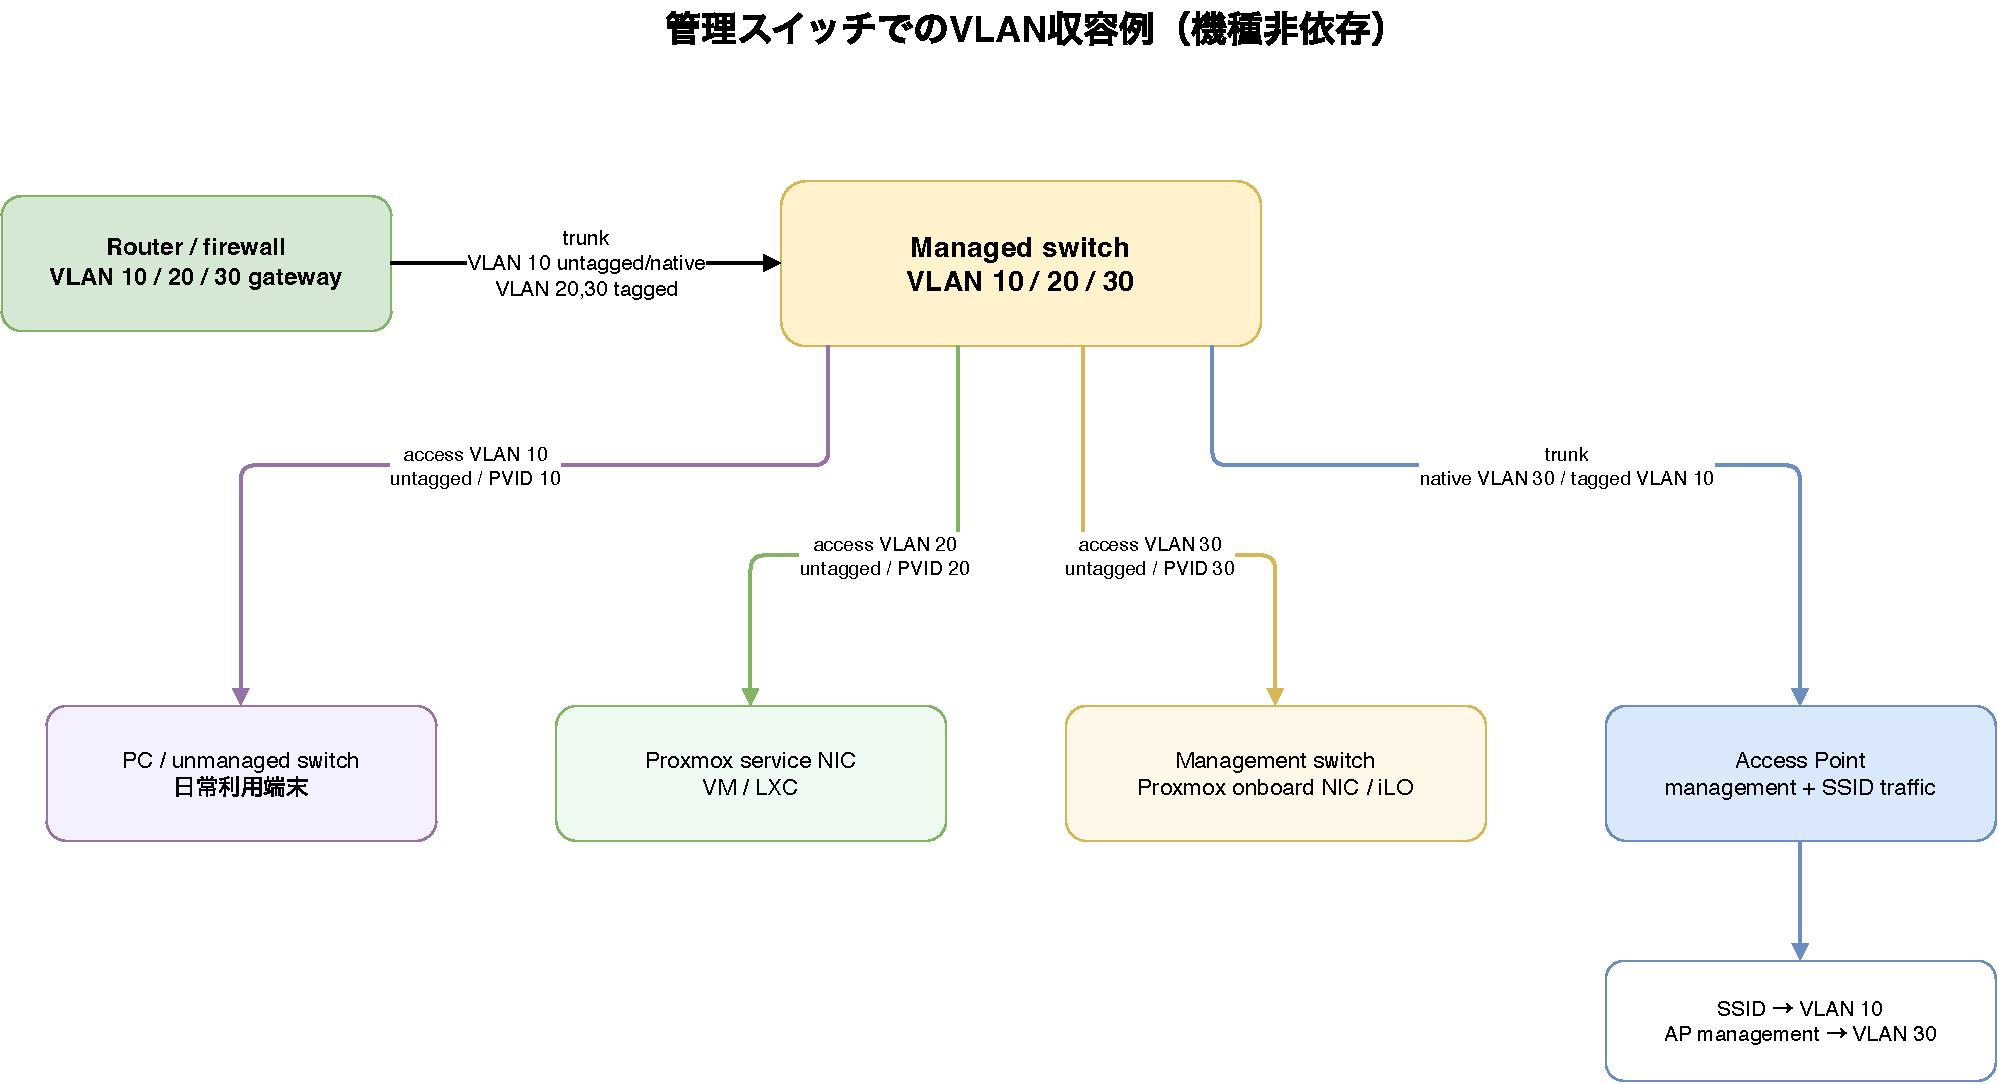
\includegraphics[width=0.98\linewidth]{media/diagrams/home-network-switch-overview.pdf}
  \caption{管理スイッチにおけるVLANの収容例。接続先に応じて\texttt{trunk}または\texttt{access}を選び、接続する両側でVLAN設定を一致させます。}
  \label{fig:managed-switch-vlan-overview}
\end{figure}

\termdefs{※ trunk: 複数VLANをまとめて通すポート。\\
※ access: 1つのVLANだけに所属するポート。\\
※ native VLAN: trunkでタグなし通信として扱うVLAN。\\
※ tagged: VLAN tag付き通信として扱う状態。}

\begin{itemize}
\item 複数VLANを扱う機器へのポートは\texttt{trunk}にして必要なVLANを\texttt{tagged}で通し、単一用途の機器へのポートは\texttt{access}にして所属するVLANを1つ指定する。
\item \texttt{native VLAN}は接続する両側で揃え、管理IPを管理用VLANへ移す場合は、変更後も管理画面へ到達できる経路を先に確保する。
\item 設定後は、各ポートのVLANへの所属、\texttt{trunk}で許可したVLAN、管理IPへの到達性を確認し、再起動後も残るよう設定を保存する。
\end{itemize}

\subsection{VM/LXC用bridgeを分け、サービスをVLAN 20へ移す}

Proxmoxでは、管理用bridgeとVM/LXC用bridgeを分けます。オンボードNICの \texttt{nic0} は管理用bridge \texttt{vmbr0} に入れ、各ノードを設計表のとおり \texttt{10.1.30.3}〜\texttt{10.1.30.5} のVLAN 30に置きます。X520-DA2の1ポート目 \texttt{nic1} は、新しく作るLinux bridge \texttt{vmbr20} に入れます。

「System」→「Network」→「Create」→「Linux Bridge」で、\texttt{Name} に \texttt{vmbr20}、\texttt{Bridge ports} に \texttt{nic1} を入れます。IPv4/CIDR、Gateway、IPv6/CIDRは空欄、Autostartは有効、VLAN awareは無効にします。HPE 5920側の接続ポートをVLAN 20の\texttt{access port}にしているため、\texttt{VLAN tag}はProxmox側で付けず、物理スイッチ側で収容します。

\installfigure[0.55\linewidth]{media/proxmox-installation/08-terumox3-vmbr20-linux-bridge-filled-form.png}{terumox3で\texttt{vmbr20}を作成する画面。このbridgeはVM/LXC用のVLAN 20通信だけを受け持ちます。}{fig:vmbr20}

保存して反映後、\texttt{vmbr0} が管理用IPを持ったまま残り、\texttt{vmbr20} が \texttt{nic1} をポートとして持っていれば意図通りです。これで、管理経路はオンボードNIC側、VM/LXCのサービス通信はX520-DA2側に分かれます。

続いて、サービス用のVM/LXCの仮想NICを \texttt{vmbr20} へ移し（VLAN Tagは空欄）、VLAN 20の固定IPを割り当てました。たとえば、AdGuard Homeは \texttt{10.1.20.22}、Zabbixは \texttt{10.1.20.27}、Crafty Controllerは \texttt{10.1.20.50} です。ほかのサービスも同じ帯域で重複しないように管理しています。

変更後は、クラスタがquorumを保っていること、3ノードがonlineのままであること、各VM/LXCが \texttt{vmbr20} を使っていることを確認します。

\subsection{home.arpaで名前解決する}

わかりやすい名前でアクセスできるよう、AdGuard HomeにDNS rewriteを登録しました。

\begin{commands}
# DNS rewriteの例。ポート番号はDNS名ではなくURL側に付ける。
terumox1.home.arpa  -> 10.1.30.3
terumox2.home.arpa  -> 10.1.30.4
terumox3.home.arpa  -> 10.1.30.5
adguard.home.arpa   -> 10.1.20.22
crafty.home.arpa    -> 10.1.20.50
\end{commands}

設定後は \texttt{dig @10.1.20.22 terumox1.home.arpa +short} のようにAdGuardへ直接問い合わせて確認します。あとは、ER8411のDHCP設定でVLAN 10/20/30の配布DNSを \texttt{10.1.20.22} にすれば、通常の端末もAdGuardを見るようになります。

自宅LANの外からTailscale経由でアクセスする場合は、\texttt{home.arpa} の名前解決を \texttt{10.1.20.22} へ転送するsplit DNSをTailscale側に設定します。

\termdefs{※ DNS rewrite: 特定の名前を指定したIPへ返すDNS側の固定登録。\\
※ split DNS: 特定ドメインだけ別のDNSサーバーへ問い合わせる設定。}

\subsection{CodexからProxmoxを操作する（ProxmoxMCP-Plus）}

最近流行りのコーディングエージェントを用いてProxmoxを操作できたら面白そうだなと思って試しました。ProxmoxMCP-Plus\cite{proxmox-mcp-plus}というOSSを使います。
\siteqrcode{ProxmoxMCP-Plus}{https://github.com/RekklesNA/ProxmoxMCP-Plus}

Codexへrootパスワードを渡すのは怖いので、Proxmox側に専用ユーザーとAPI tokenを作ります。普段使うtokenは読み取りと低リスク操作に絞り、Administrator tokenは別にして必要なときだけ使うことにしました。tokenなら用途ごとに権限を分けられ、不要になったときはパスワードを変更せずに失効できます。

\termdefs{※ API token: パスワードの代わりにアプリへ渡す認証用の鍵。\\
※ role: Proxmoxで複数の権限をまとめたもの。\\
※ ACL: どのユーザーが、どの範囲で、どのroleを使えるかを決める設定。}

\subsubsection*{常用ユーザーとAPI tokenを作る}

ProxmoxのWeb UIで「Datacenter」→「Permissions」→「Users」→「Add」を開き、\texttt{codex@pve} を作ります。続いて「API Tokens」→「Add」で、同じユーザーに \texttt{codex} というtokenを作ります。\texttt{Privilege Separation} は有効にします。表示されるtoken secretは一度しか確認できないため、その場でコピーして安全な場所へ保存します。

CLIで作る場合は、ProxmoxホストのShellで次のように実行できます。token作成時に表示された値は原稿やGitへ書きません。

\begin{commands}
# Codex専用ユーザーと、権限分離した読み取り用tokenを作る。
pveum user add codex@pve --comment "Codex MCP automation user"
pveum acl modify / -user codex@pve -role PVEAuditor
pveum user token add codex@pve codex -privsep 1 \
  --comment "Codex MCP read-only token"
pveum acl modify / -token 'codex@pve!codex' -role PVEAuditor

# ユーザー本体とtokenに付いた権限を確認する。
pveum user permissions codex@pve
pveum user token permissions codex@pve codex
\end{commands}

ここで注意するのが \texttt{Privilege Separation} です。有効にしたtokenでは、元ユーザーとtokenの両方へ権限を付ける必要があります。最初はtoken側だけに \texttt{PVEAuditor} を付けましたが、Codexから見えたのはノード一覧だけで、ストレージやVM/LXCの一覧は空でした。最終的に、DatacenterのPermissionsへ次の2つが入った状態で取得できました。

\begin{commands}
# Pathは /、Propagateは有効にする。
/  codex@pve        PVEAuditor  true
/  codex@pve!codex  PVEAuditor  true
\end{commands}

\subsubsection*{ProxmoxMCP-Plusの接続設定を作る}

ProxmoxMCP-Plusのexampleを \texttt{config.json} としてコピーし、接続先、ユーザー、token名、token secretを書き換えます。我が家の最初の接続先は \texttt{terumox1} の管理IP \texttt{10.1.30.3:8006} です。

\begin{commands}
# exampleをコピーし、ローカル専用の設定ファイルを作る。
cp proxmox-config/config.example.json \
  proxmox-config/config.json
nano proxmox-config/config.json
\end{commands}

設定する主な項目は次のとおりです。\texttt{token\_value} には、先ほどコピーしたsecretを入れます。

\begin{commands}
"proxmox": {
  "host": "10.1.30.3",
  "port": 8006,
  "verify_ssl": false,
  "service": "PVE"
},
"auth": {
  "user": "codex@pve",
  "token_name": "codex",
  "token_value": "ここにtoken secret"
},
"security": {
  "dev_mode": true
}
\end{commands}

初期状態のProxmoxは自己署名証明書を使うため、最初の疎通確認では \texttt{verify\_ssl=false} にしました。ProxmoxMCP-Plusでは、この設定を使う場合に \texttt{security.dev\_mode=true} も必要です。長期運用では証明書を信頼できる状態にして、\texttt{verify\_ssl=true} と \texttt{dev\_mode=false} へ戻します。

secret入りファイルは自分だけが読めるようにし、Gitへ追加しません。

\begin{commands}
# token secretを含む設定ファイルの権限を制限する。
chmod 600 proxmox-config/config.json
git status --short proxmox-config/config.json
\end{commands}

\subsubsection*{Codexへ常用MCPを登録する}

Codexの \texttt{config.toml} には、ProxmoxMCP-Plusを \texttt{uvx} で起動するMCPサーバーを登録します。読み取り系だけを自動承認し、起動、停止、snapshot作成などの状態変更は毎回確認する設定にしました。削除、rollback、restore、SSH経由のcommand executionは常用側へ公開しません。

\begin{commands}
# ~/.codex/config.toml に追記する。
# 同名の見出しがある場合は重複させず、中身を置き換える。
[mcp_servers.proxmox]
command = "uvx"
args = ["proxmox-mcp-plus"]
env = { PROXMOX_MCP_CONFIG = "/path/to/proxmox-config/config.json" }
default_tools_approval_mode = "prompt"
enabled_tools = [
  "get_nodes",
  "get_cluster_status",
  "get_storage",
  "get_vms",
  "get_containers",
  "list_snapshots",
  "start_vm",
  "start_container",
  "stop_container",
  "create_snapshot",
  "list_jobs",
  "get_job",
  "poll_job"
]

# 一覧取得などの読み取り系だけを自動承認する。
[mcp_servers.proxmox.tools.get_nodes]
approval_mode = "approve"

[mcp_servers.proxmox.tools.get_cluster_status]
approval_mode = "approve"

[mcp_servers.proxmox.tools.get_storage]
approval_mode = "approve"

[mcp_servers.proxmox.tools.get_vms]
approval_mode = "approve"

[mcp_servers.proxmox.tools.get_containers]
approval_mode = "approve"

[mcp_servers.proxmox.tools.list_snapshots]
approval_mode = "approve"
\end{commands}

\texttt{stop\_vm} はProxmoxMCP-Plusのtool定義上force stopになるため、常用側の \texttt{enabled\_tools} から外しました。VMを停止するときは、まずguest OSを正常終了させるgraceful shutdownを使います。

\subsubsection*{読み取りだけで接続を確認する}

設定を反映するためCodexを再起動し、最初は次のように変更を禁止したうえで一覧取得だけを依頼しました。

\begin{commands}
# Codexへの最初の依頼。
Proxmoxのnode、storage、VM、LXC一覧を取得して。
変更操作はしないで。
\end{commands}

権限を修正したあとの取得結果は次のとおりです。3ノード、2つのstorage、VM 1台、LXC 13台を読み取れました。

\begin{commands}
nodes:
terumox1 online
terumox2 online
terumox3 online

storage:
local-lvm
local

VM:
100 docker

LXC:
101 adguard
102 cloudflared
103 wireguard
104 tailscale
105 homeassistant
106 crafty-controller
107 proxmox-backup-server
108 ubuntu
109 n8n
110 zabbix
111 upsnap
112 netbox
113 bentopdf
\end{commands}

ここまで読めることを確認してから、snapshot作成、VM/LXCの起動、LXCのgraceful shutdown、job確認を追加しました。変更操作を頼むときは、先にnode、VMID/CTID、名前、現在状態を取得し、対象を確認してから実行します。

\subsubsection*{管理作業用tokenを分離する}

すべての設定作業をCodex経由で行う場合でも、常用tokenをAdministratorへ昇格させません。\texttt{codex-admin@pve} と \texttt{codex-admin@pve!admin} を別に作り、ユーザー本体とtokenの両方へAdministratorを付けます。

\begin{commands}
# DatacenterのPermissionsで確認する管理用ACL。
/  codex-admin@pve        Administrator  true
/  codex-admin@pve!admin  Administrator  true
\end{commands}

管理用のsecretは \texttt{config.admin.json} へ保存し、常用設定と混ざらないようにします。Codex側でも \texttt{proxmox\_admin} という別名で登録し、読み取りを含むすべてのtoolを実行前確認にしました。

\begin{commands}
# ~/.codex/config.toml に追加する管理作業用MCP。
[mcp_servers.proxmox_admin]
command = "uvx"
args = ["proxmox-mcp-plus"]
env = { PROXMOX_MCP_CONFIG = "/path/to/proxmox-config/config.admin.json" }
default_tools_approval_mode = "prompt"
\end{commands}

管理用namespaceでは、削除、rollback、restore、ISOやbackupの削除、command execution、VMのforce stopまで見えます。使う前に対象、目的、戻し方を確認し、作業後はMCP設定またはtokenを無効にします。実際の確認では、\texttt{terumox-cluster} がquorumを保ち、3ノードがonlineであることまで読み取れました。

設定ファイル一式と、token secretを履歴へ残さず保存する補助スクリプトは、原稿付属の補足資料にも載せています。
\siteqrcode{ProxmoxMCP-Plus 完全設定メモ}{https://github.com/terudoru/edp2026-article/blob/main/supplements/proxmox-mcp-plus-setup.md}


\subsection{Zabbixで監視する}

サーバーが増えてくると監視が欲しくなるので、Zabbixを導入しました。

まずはミライサーバーの記事を見ながら、Zabbix本体のインストール、DBの作成などを行うとよいです\cite{miraiserver-zabbix-ubuntu}。

\siteqrcode{Zabbix本体の導入手順}{https://www.miraiserver.ne.jp/column/about_zabbix-install-ubuntu/}

日本語を選択できない場合は、\texttt{language-pack-ja} を導入して \texttt{ja\_JP.UTF-8} を生成し、システムの言語設定へ反映します。

Zabbixが立ち上がったら、次はProxmoxを監視対象として追加します。Proxmox VEはAPIを備えており、Zabbix側にも \texttt{Proxmox VE by HTTP} テンプレートがあります。ITログの記事では、Proxmox側で監視用ユーザーを作り、API tokenを発行し、Zabbix側でホスト追加とマクロ設定を行う流れが画面付きでまとまっています\cite{filewo-proxmox-zabbix}。

\siteqrcode{Proxmox VEをZabbixで監視する手順}{https://www2.filewo.net/wordpress/2025/05/19/4294/}

\termdefs{※ API token: パスワードの代わりにアプリへ渡す認証用の鍵。\\
※ template: Zabbixで監視項目や取得方法をまとめたひな形。\\
※ SNMP: スイッチやルーターから状態を読むためによく使われる監視用プロトコル。}

\subsection{余談：IOMMUとPCI passthrough}

ほかにも、ルーターVMを試す過程でIOMMUやPCI passthroughを触りました。このへんは本筋から外れるため、設定手順、確認コマンド、検証結果をGitHubに載せておきます。
\siteqrcode{Proxmox IOMMU確認・設定メモ}{https://github.com/terudoru/edp2026-article/blob/main/supplements/iommu-notes.md}


\section{おわりに}

このままだと締まりが悪いので、好きなコンテンツの二次元コードを貼って終わりにしたいと思います。

\begin{center}
\qrcode[height=11mm]{https://www.ohayo-milk.co.jp/dessert/14050.html}\hspace{2em}%
\qrcode[height=11mm]{https://www.youtube.com/@GIFGAS}\hspace{2em}%
\qrcode[height=11mm]{https://www.youtube.com/@darkfantasy7395}\hspace{2em}%
\qrcode[height=11mm]{https://www.youtube.com/@Nujabes19740207}\hspace{2em}%
\qrcode[height=11mm]{https://www.youtube.com/watch?v=C6gl9ngTHc8}
\end{center}


\phantomsection
\addcontentsline{toc}{section}{参考にしたサイト}
\begin{thebibliography}{99}
\small
\setlength{\itemsep}{0.12\baselineskip}
\setlength{\parsep}{0pt}
\bibitem{proxmox-ve}
Proxmox Server Solutions GmbH,
``Proxmox Virtual Environment - Open-Source Server Virtualization Platform'',
\biburlqr{https://www.proxmox.com/en/products/proxmox-virtual-environment/overview}

\bibitem{proxmox-helper-scripts}
Community Scripts,
``Proxmox VE Helper-Scripts'',
\biburlqr{https://community-scripts.github.io/ProxmoxVE/}

\bibitem{katori-adguard-home}
katori\_m,
``AdGuard Homeで広告ブロック\&お手軽内部ネットワーク用DNSを作ろう(ついでに冗長化)'',
Qiita,
\biburlqr{https://qiita.com/katori_m/items/02aef27024b848b160a4}

\bibitem{miraiserver-zabbix-ubuntu}
ミライサーバーのススメ,
``はじめてのZabbix構築 Ubuntu24.04/22.04で監視サーバーを立ち上げる実践ガイド'',
\biburlqr{https://www.miraiserver.ne.jp/column/about_zabbix-install-ubuntu/}

\bibitem{filewo-proxmox-zabbix}
tukapiyo,
``Proxmox VEをZabbixで監視する'',
ITログ,
\biburlqr{https://www2.filewo.net/wordpress/2025/05/19/4294/}

\bibitem{wildrick-proxmox-cluster-remove}
wildrick,
``Proxmoxクラスタからノードを削除する手順'',
\biburlqr{https://note.com/wildrick/n/nbcfdbb8dffaa}

\bibitem{proxmox-mcp-plus}
RekklesNA,
``ProxmoxMCP-Plus'',
\biburlqr{https://github.com/RekklesNA/ProxmoxMCP-Plus}

\bibitem{reddit-proxmox-standalone-node}
w453y,
``[Guide] How I turned a Proxmox cluster node into standalone (without reinstalling it)'',
Reddit,
\biburlqr{https://www.reddit.com/r/Proxmox/comments/1k4slor/guide_how_i_turned_a_proxmox_cluster_node_into/}

\bibitem{proxmox-forum-pve-ssl-pem}
karlsiu1,
``Joining Cluster pve-ssl.pem error'',
Proxmox Support Forum,
\biburlqr{https://forum.proxmox.com/threads/joining-cluster-pve-ssl-pem-error.131263/}

\bibitem{reddit-proxmox-enable-iommu}
Important\_Reserve460,
``[Guide] How to enable IOMMU for PCI Passthrough'',
Reddit,
\biburlqr{https://www.reddit.com/r/Proxmox/comments/1brl7vw/guide_how_to_enable_iommu_for_pci_passthrough/?tl=ja}

\bibitem{proxmox-forum-x520-iommu-groups}
zayigo,
``Intel X520-DA2 IOMMU groups'',
Proxmox Support Forum,
\biburlqr{https://forum.proxmox.com/threads/intel-x520-da2-iommu-groups.118261/}

\bibitem{tenforward-enable-sr-iov}
TenForward,
``SR-IOVを有効にする'',
\biburlqr{https://tenforward.hatenablog.com/entry/20111206/1323171401}

\bibitem{enokiko-proxmox-intel-nic-sr-iov}
えのきこ,
``ProxmoxでIntel NICをSR-IOV'',
note,
\biburlqr{https://note.com/enokiko/n/n4b4b4e4c399b}
\end{thebibliography}
